\documentclass[12pt,a4paper]{report}
\usepackage[utf8x]{inputenc}
\usepackage{amsmath}
\usepackage{amsfonts}
\usepackage{amssymb}
\usepackage{graphicx}
\usepackage{ragged2e}
\usepackage{float}
\usepackage{appendix}
\usepackage{listings}
\usepackage[left=2cm,right=2cm,top=2cm,bottom=2cm]{geometry}
\author{Md. Hasanuzzaman Noor}
\title{An Efficient Link Layer Handoff Procedure in Infrastructure Wireless Mesh Nerworks}
% arara: indent
\begin{document}
\maketitle

\newpage
\begin{center}
\section*{Acknowledgment}
\justify
First and foremost, I would like to thank God Almighty for giving me the strength to finish this work. The satisfaction that accompanies the successful completion of this thesis would be incomplete without the mention of people whose ceaseless cooperation made it possible, whose constant guidance and encouragement crown all efforts with success. I am grateful to my honorable project Supervisor Mir Md. Saki Kowsar, Assistant Professor, Department of Computer Science and Engineering, Chittagong University of Engineering and Technology, for the guidance, inspiration and constructive suggestions which were helpful in the preparation of this project. I also convey special thanks and gratitude to Professor Dr. Kaushik Deb, honorable head of the Department of Computer Science and Engineering for his kind advice.I would also like to extend my gratitude to all of my teachers for their valuable guidance in every step of mine during the four years of learning stage. Finally I would like to thank my friends, senior, juniors and the staffs of the department for their valuable suggestion and assistance that has helped in successful completion of the project. 
\end{center}
\newpage

\begin{center}

\section*{Abstract}
\justify
Wireless Mesh Networks (WMN) usually provides internet access to a large area, which is from university campus to city scale. In order to provide an uninterrupted internet experience to a mobile client, a process called handoff is required to maintain the network connection. Ideally, handoff should be completely transparent to mobile users. A critical application like VoIP will require a handoff capability that transfers a call from one mesh node (MN) to another in less than 50 msec. However the current IEEE 802.11 standards do not address the handoff well. Studies have revealed that standard handoff on IEEE 802.11 WLANs incurs a latency of the order of hundreds of milliseconds to several seconds. Moreover, the discovery step in the handoff process accounts for more than 99\% of this latency. The study addresses the latency in the discovery step by introducing an efficient and powerful client-side scan technique which optimizes the discovery step with an efficient method. The feasibility of the proposed scheme to support fast handoff in WMNs has been demonstrated through computer simulations under different network conditions. The results from the simulations show that the latency associated with handoff can be reduced by using this technique.

\end{center}
\tableofcontents
\listoffigures
\chapter{Introduction}
An infrastructure Wireless Mesh Network is composed of a combination of static mesh routers (MRs) and mobile mesh nodes (MNs). In a typical WMN, MRs form a wireless multi-hop backbone network. Some MRs serve as the wireless access points (APs) to provide wireless mesh backbone entries to MNs. Some MRs, called gateway MRs (GW), are connected to the Internet via wired links and serve as the Internet entry points to other MRs via multi-hop wireless links. MNs can move freely in WMNs when communicating with correspondent nodes (CNs) by means of handoffs between different APs.This chapter contains some introductory information on handoff in wireless mesh network, motivation of our work, challenges of implementing our work and our objectives.
\section{Handoff in Wireless Mesh Network}
One of the main characteristics of mesh networks is that they have only a few wireless gateways (GWs) connected to a wired network while the wireless routers (MR) provide Network access to mobile. Within the range of a given wireless router, the client may move freely, but as it moves away from the wireless router and closer to another, it should handover all its open connections to the new one to preserve network connectivity [1]. Ideally the handover should be completely transparent to mobile clients with no interruption, loss of connectivity, or degradation of voice quality if VoIP communications are involved. Handover is the essential component for dealing with the mobility of clients. It guarantees the continuity of the wireless services when the client moves across the boundaries.There are four different types of handovers in Wireless Mesh Network [1]. They are:
\begin{itemize}
\item 
Intra-system HO: occurs within one system. It can be further divided into Intra-frequency HO and Inter-frequency HO. Intra-frequency occurs between cells belonging to the same Wireless Mesh Network carrier, while Inter-frequency occurs between cells operate on different Wireless Mesh Network carriers.
\item 
Inter-system HO: takes places between cells belonging to two different Radio Access Technologies(RAT) or different Radio Access Modes (RAM).
\item 
Hard HO: is a category of HO procedures in which all the old radio links of a mobile are release dbefore the new radio links are established. Hard handover can take place as intra or inter-frequency handover.
\item 
Soft HO: During soft handover, a mobile simultaneously communicates with two (2-way SHO)or more cells belonging to different APs of the same wireless gateway (intra-WG) or different wireless gateway (inter-WG). Soft handover is only possible within one carrier frequency and therefore, it isintra-frequency handover processes.
\end{itemize}
\section{Motivation of the Work}
Much of the work to date [2-4] in the area of handoff in IEEE 802.11 wireless networks has been concerned with essentially trying to duplicate the successful handoff mechanisms that already exist in cell phone networks when a mobile device roams between base stations.  A cell phone handoff must be quick enough to support full-duplex voice communication without a perceivable gap in either voice stream.Previous studies on seamless mobility in wireless mesh networks can be divided into two different categories: MAC layer handoff and network layer handoff. MAC layerhandoff is often referred to as micro-mobility while network layer handoff is referred to as macro-mobility. Surveys addressing all of these areas are reviewed by Akyildiz et al. in [5]. Improvements have been shown in the previous studies [3-4, 6-7], but most ofthem are not specifically focused on WMNs or only address centrally controlled solutions which are expensive to deploy.
\section{Challanges}
Wireless Mesh Networks (WMNs) are a new architecture intended to provide a cost effective high-bandwidth network over a large coverage area. In recent years, WMNs have emerged as a promising solution to provide low cost access networks that extend Internet access and other networking services. A significant application for WMNs is VoIP. Wireless VoIP applications are beginning to emerge in the business market and IP Telephony revenues will more than double by 2013, compared to 2008, according to research from In-Stat [8]. Voice users are far more mobile than data users and will require a handoff capability that can transfer a call from one mesh node (MN) to another in less than 50 msec. [9]. Handoff introduces temporary variation in the delay – more appropriate to consider as jitter rather than delay. According to the IEEE 802.11 standard, the handoff process can take from a few hundred milliseconds to several seconds which is unacceptable for VoIP users. Ideally, handoff should be completely transparent to mobile VoIP users, however the current IEEE 802.11 standard does not address this issue properly. In July 2008, the IEEE published the final specification for the IEEE 802.11r-2008 standard [10], also known as Fast Basic Service Set Transition which is an amendment to the IEEE 802.11 standard that supports fast handoff between access points by introducing the Fast BSS Transition (FT) mechanism. The FT mechanism addresses two classes of network 2 infrastructures from a QoS perspective, but it still does not address the core questions of when and where a station (STA) will handoff to.
\section{Contribution of the Work}
The objective of this thesis is to develop a MAC layer handoff scheme to provide fast handoff in WMNs. After a study and analysis of the IEEE 802.11 standard handoff procedure, the handoff process was divided into two phases: discovery phase (discovery latency) which is used to discover the available APs/MNs and the execution phase whichincludes two authentication and (re)association phases. A fast handoff management scheme have been developed to provide a novel use of the channel scanning technique by employing open system authentication in both Passive Handoff and Active Handoff. This handoff scheme may be implemented by upgrading the software on the client side, no hardware upgrade is required. NS-3 simulations were used in order to verify the feasibility of the proposed scheme.The results presented in chapter 5 indicate that the latency associated with handoff canbe reduced by using the proposed technique. The performance of the proposed scheme was also analyzed. The results show that the scheme continued to successfully operate under different network conditions.
\section{Organization of the Project}
The remainder of the report is organized as follows. In the next chapter, an overview of our project related terminologies and contains brief discussion on previous works that is already implemented with their limitations. Chapter three describes the working procedure of our proposed system. In Chapter 4, we have illustrated our implementation of the project in details. Chapter 5 focuses on the experimental result of the proposed system. The thesis concludes with a summary of research contributions and future plan of our work in chapter 6. This thesis contains an appendix intended for persons who wish to explore the source code. 
\chapter{Literature Review}
Handoff support is an essential issue to ensure continuous communications in wireless mesh networks (WMNs). The handoff performance in WMNs can be largely degraded by the long queueing delay and medium access delay at each mesh router, especially when the backbone traffic volume is high. In this chapter we present studies on the terminologies related to the project which are important to understand. This chapter also contains brief discussion on previous works that is already implemented along with their limitations.
\section{Wireless Mesh Network}
The Wireless Mesh Network (WMN) [11] is a new architecture for wireless networking that incorporates existing and new radio technologies defining the overall structure, components and the inter-relationships between devices in the network. This means that mesh networking technology can be applied to practically any radio scheme, effectively allowing the best radio technology to fit the desired application: Personal area networks(i.e.Bluetooth, UWB), local area networks(i.e. Wi-Fi), and wide area networks(i.e. WiMaxand cellular). WMN is set to become the predominant wireless network technology for next generation networks as it has many advantages compared to traditional wireless networks:
 \begin{itemize}
 \item 
 Self Organizing - each node determines the routing paths for itself, saving time and effort in administration.
\item 
 Wide Coverage - multi-hop networks extend the communications coverage around obstacles and over greater distances.
\item 
 Scalable – The size of the network may be increased by simply adding more nodes.
The routing configuration is automatic, and there is no exponential rise in complexity as the network grows.
\item 
 Network Resilience - The self-organizing functions run continuously, so when changes occur in connections and reception (i.e. when the network topology changes) the mesh will automatically re-route around blockages in real time.
\item
Cost effective – Less cabling need compare to traditional wireless networks.
\end{itemize}
A WMN is a collection of wireless devices, typically operating as APs that utilize special routing algorithms to dynamically adapt to changes in the network. These changesm ay be triggered by factors such as environmental changes, movement of the Mesh Nodes (MNs) or even failure of the MNs due to loss of electrical power. This project is particularly interested in WMNs based on the IEEE 802.11 standards where at least one MN has a wired Internet connection to act as a network gateway. The other MNs connect to the gateway MN in order to gain access to the backbone network. An example of an IEEE802.11 mesh network is illustrated below in Figure.2.1 [11].All of the MNs individually create Basic Service Sets (BSS) or hotspots and collectively create an Extended Service Set (ESS) or network coverage area. Usually, there will be a degree of overlap between the hotspots of different MNs. Mobile users roaming within the network coverage area will have to undergo handoff from one MN to another in order to preserve their network connectivity. The reason why user wants to use WMN compare to telecom network (i.e. EDGE, 3G, upcoming 4G) for VoIP calls is because 802.11 based WMN is cheaper to use and in most of the case is free of charge.

\subsection{Network Architecture}
WMNs consist of two types of nodes: mesh routers and mesh clients. Other than the routing
capability for gateway/repeater functions as in a conventional wireless router, a wireless mesh router contains additional routing functions to support mesh networking. To further improve the flexibility of mesh networking, a mesh router is usually equipped with multiple wireless interfaces built on either the same or different wireless access technologies. Mesh clients also have the necessary functions for mesh networking, and thus can also work as a router in WMN. However, gateway or bridge functions do not exist in these nodes. In addition, mesh clients usually have only one wireless interface. As a consequence, the hardware platform and the software for mesh clients can be much simpler than those for mesh routers. Mesh clients have a greater variety of devices compared to mesh routers. They can be a laptop/desktop PC, pocket PC, PDA, IP phone, RFID reader, BACnet (Building Automation and Control network) controller, and many other devices
The architecture of WMNs can be classified into three main groups based on the functionality of the nodes.
\subsubsection{Infrastructure/Backbone WMNs}
Infrastructure/Backbone WMN includes mesh routers that form an infrastructure for clients that connect to them. The WMN infrastructure/backbone can be built using various types of radio technology, in addition to the heavily used IEEE 802.11 technology. The mesh routers form a mesh of self-configuring, self-healing links among themselves. With gateway functionality, mesh routers can be connected to the Internet. This approach, also referred to as infrastructure meshing, provides backbone for conventional clients and enables the integration of WMNs with existing wireless networks, through gateway/bridge functionalities in mesh routers.
Infrastructure/Backbone WMNs are the most commonly used type. For example, community and neighborhood networks can be built using infrastructure meshing.The mesh routers are placed on the roofs of houses in a neighborhood, and these can serve as access points for users in homes and along the roads. Typically, two types of radio are used in the routers, i.e., for backbone communication and for user communication. The mesh backbone communication can be established using long-range communication techniques including, for example, directional antennas.
\begin{figure}[H]
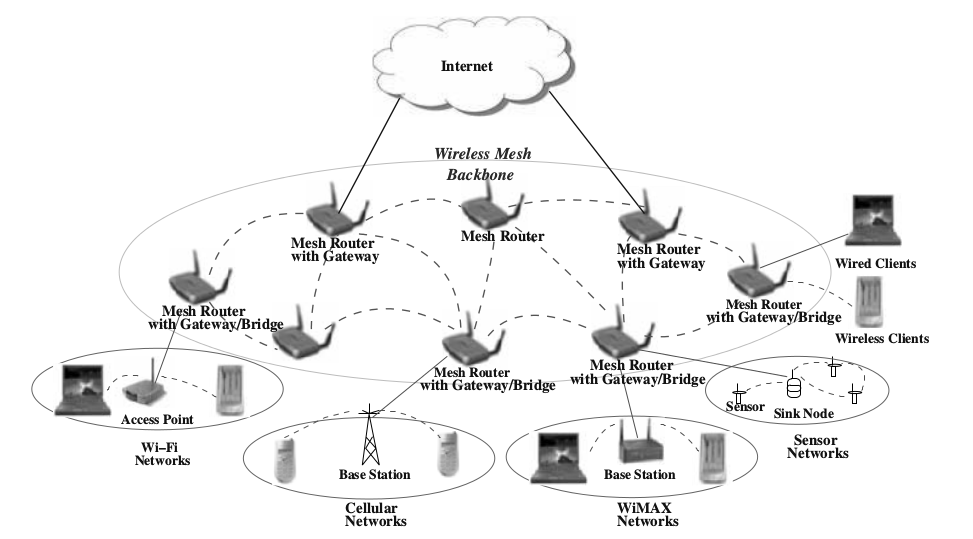
\includegraphics[scale=.5]{thesis-pic/infrastructure-mesh.png}
\caption{Infrastructure WMN}
\end{figure}
\subsubsection{Client WMNs}
Client meshing provides peer-to-peer networks among client devices. In this type of architecture, client nodes constitute the actual network to perform routing and configuration functionalities as well as providing end-user applications to customers. Hence, a mesh router is not required for this type of network.
\begin{figure}[H]
\centering
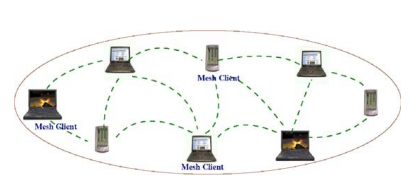
\includegraphics[scale=1]{thesis-pic/client-wmn.png}
\caption{Client WMNs}
\end{figure}




\subsubsection{Hybrid WMNs}
This architecture is the combination of infrastructure and client meshing. Mesh clients can access the network through mesh routers as well as directly meshing with other mesh clients. While the infrastructure provides connectivity to other networks such as the Internet, Wi-Fi, WiMAX, cellular and sensor networks, the routing capabilities of clients provide improved connectivity and coverage inside the WMN.
\begin{figure}[H]
\centering
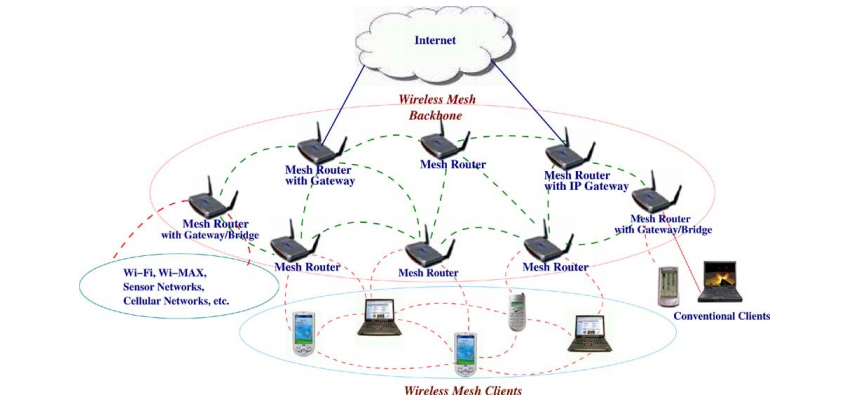
\includegraphics[scale=0.75]{thesis-pic/hybrid-wmn.png}
\caption{Hybrid WMNs}
\end{figure}

\subsection{Application}
Research and development of WMNs is motivated by several applications which clearly
demonstrate the promising market, but, at the same time, these applications cannot be
supported directly by other wireless networks such as cellular systems, ad hoc networks,
wireless sensor networks, standard IEEE 802.11, etc. In this section, we discuss these
applications.
\begin{itemize}
\item Broadband home networking
\item Community and neighborhood networking
\item Enterprise networking
\item Metropolitan area networks (MAN)
\item Transportation systems
\item Building automation
\item Health and medical systems
\item Security surveillance systems
\end{itemize}
In addition to the above applications, WMNs can also be applied to spontaneous
(emergency/disaster) networking and P2P communications. For example, wireless networks
for an emergency response team and firefighters do not have in-advance knowledge of
where the network should be deployed. By simply placing wireless mesh routers in
desired locations, a WMN can be quickly established.
For a group of people holding
devices with wireless networking capability, e.g., laptops and PDAs, P2P communication
anytime anywhere is an efficient solution for information sharing. WMNs are able to meet this demand. These applications illustrate that WMNs are a superset of ad hoc networks, and thus, can accomplish all functions provided by ad hoc networking.
\section{Handoff in 802.11 WMN}
A handoff occurs in an IEEE 802.11WMN [14] when a mobile STA moves beyond the radio range of one MN and enters another coverage area at the MAC layer (e.g. where a STA moves from one BSS to another BSS or where both BSS are belonging to same ESS.) or when a mobile STA finds another AP/MN having a stronger beacon signal than the current one. During the handoff, management frames are exchanged between the STA and the MN. Consequently, there is a latency involved in the handoff process during which the STA is unable to send or receive traffic. The original design of the IEEE 802.11 standards just considered the handoff signaling where the handoff procedure can be divided into three phases: discovery, authentication and association/reassociation [12].
\subsection{Link Layer Handoff}
When a station moves out of range of an AP, it triggers a link layer handoff to search for and reassociate witha new AP. The exact condition that triggers a handoff is implementation specific. For example, a client can initiate a handoff when it fails to communicate withthe AP it is currently associated with. Or, the handoff initiation can be more proactive. For example, the client can continuously do signal strength measurements for the beacon messages from APs that it is hearing on the current channel. If the signal strength of the AP it is currently associated with falls below a threshold and the signal strength from another AP is sufficiently higher,the client may trigger a handoff to the second AP. These conditions avoid ping-ponging between two Aps due to slight fluctuation of signal strengths .Handoff is often associated with probing. Probing proactively seeks APs to associate with instead of waiting to hear beacon signals. This is because beacon intervals can often be too high (e.g., more than 100ms). Also, there may not be any AP to associate to in the current channel. In probing, the client broadcasts a probe request frame. APs on the same channel respond with probe response frames. The client waits for certain amount of time (probe-wait time) to collect all the probe responses. Then, the client can switch to other channels to probe. After probing a set of channels (possibly all available channels), the client selects one AP with the best SINR (signal-to-noise ratio) based on the probe responses.After probing is complete, the station authenticates with the new AP. Following successful authentication,the station initiates reassociation with the new AP toexchange information about the connection such as transmissionrates, beacon intervals, etc. It sends a reassociation request frame to the AP that responds with a reassociation response frame. At this point, the linklayer handoff completes.
\subsection{Discovery}
Discovery is the process used to allow the STA identify the available MNs within the RF coverage range. Two methods are defined in the IEEE 802.11 standard, namely passive scanning and active scanning. In passive scanning, the STAs do not transmit any frames on the medium and instead wait and listen to each available channel for beacon frames which are broadcasted periodically by the MNs. Usually, the beacon frame transmission period is configured at 100 ms, which makes the timescale of MN discovery on the scale of a second since there are 11 available channels in United States and 13 available channels in Europe [15], and a STA must scan each channel in turn. In active scanning, in order to determine whether a MN is operating on a particular channel, a STA periodically broadcasts probe request frames on a particular channel. When an AP receives a probe request, it replies with a probe response frame. As with passive Scanning, the STA must scan all available channels in turn. The time required (or latency) to scan one channel depends on two parameters: MinChannelTime and MaxChannelTime. Both of these are measured in steps of a TU which corresponds to a time interval of 1024 microseconds. They control the duration of scanning in each channel. MinChannelTime defines the minimum time required to scan one channel to guarantee the reception of a Probe Response frame. If a STA waits during MinChannelTime without receiving any Probe Response after broadcasting a Probe Request, it assumes that there is no AP available in this channel. On the other hand, MaxChannelTime represents the time required to guarantee the reception of the Probe Response frames from multiple APs available in the same channel. If a STA receives a Probe Response during MinChannelTime after broadcasting Probe Request, it must extend its waiting time to MaxChannelTime in case more Probe Responses might arrive in the same channel. The IEEE standard does not specify their values, however typical values are suggested from previous empirical studies [16-17] as shown below  
$$MinChannelTime = DIFS + (aCWmin× aSlotTime)$$ 
Where aCWmin is the maximum number of slots in minimum contention window, and aSlotTime is the length of a slot. According to the analysis carried out in [16], it suggests an ideal value of this parameter lies between 1 ms [16] and 7 ms [17].
MaxChannelTime is suggested to be set to approximately 11 ms [16-17]. Another issue in the discovery phase is the channel switching delay. This overhead is a characteristic of the network interface design and reflects the time required to switch to a new frequency, resynchronize and start demodulating packets. Channel switching delay varies considerably across implementations from a maximum of 19 ms (12 ms to switch and 7 ms to resynchronize) for Intersil Prism2-based NICs to just over 5 ms for Atheros 5212-based NICs according to previous study [4]. Since this cost is per channel it adds considerable delay to the overall scanning process.
\subsection{Authentication}
Authentication is the phase used to verify the identities involved between a MN and a STA and to bring the wireless link up to the assumed physical standards of a wired link.The IEEE 802.11 standard defines two authentication algorithms: open system and shared key authentication.Open system authentication is the default authentication algorithm and any STA tha trequests authentication with this algorithm may become authenticated if the MN uses open system authentication. Open system authentication involves two step authentication transaction. The first step is the identity assertion and request for authentication and thesecond step is the authentication result. If the result is successful, the STA is mutually authenticated with MN. The minimum time required for authentication is two RTTs (RoundTrip Times) for open system authentication. RTT is the time corresponding to the transmission time of a probe request frame and an ACK response frame between two nodes [18]. Four timestamps are required to calculate the RTT using Equation (2.1), due to thepacket process delays. 
$$RTT = (T21-T11) + (T12-T22)$$
This study assumes that T11 is the timestamp of the probe request frame that is transmitted from Node A, T21 is the time that the request frame from Node A is received by Node B, T22 and T21 are similar to T11 and T21. RTT depends on anumber of factors that includes the network load, interference and contention.Shared key authentication is the same as open system authentication which allows any STAs to establish a link connection, but only a STA who knows the shared secret key can receive encrypted data. Shared key authentication involves a four step authentication transaction. The first step is identity assertion and request for authentication and the second step is a challenge text sent back to the STA, the third step requires the STA to send encrypted challenge text back to the MN, and the final step is the authentication result. Ifthe encrypted challenge text is correct, the STA is mutually authenticated with MN. The minimum time required for shared key authentication is four RTTs.
\subsection{ Association/Reassociation}
Association is the process that follows after a successful authentication where the STA is assigned a proper association identity and the required resources by the new MN. Reassociation is a service that is invoked to move a current association from one MN to another. The minimum time required for both association and reassociation is four RTTs. Association/Reassociation represents the end of the handoff process in MAC layer.
\subsection{ Handoff Procedure and Delay}
Figure 2.6 and Figure 2.7 [19-20] illustrate the basic handoff procedures for both passive scanning and active scanning respectively. The two procedures show the relevant delay associated with each step in the handoff procedure. The overall delay is the summation of scanning delay, authentication delay and association/reassociation delay.
\section{MAC Management Frames in Handoff Process}
\subsubsection{Beacon Frame}
The beacon frame[12] is one of the more important IEEE 802.11 WLAN management frames.Beacon frames are broadcasted periodically by the AP/MN in an infrastructure BSS to announce the presence of a WLAN. In IBSS networks, the transmission of beaconframes is distributed among the STAs.The beacon interval indicates the time interval between beacon transmissions. Thebeacon interval is expressed in TU (Time Unit) [12] which is defined as a measurement of Time equal to $1024 \mu s$ in the IEEE 802.11 standard. It is a configurable parameter in theAP/MN and by default is configured as 100 TU (100 ms). 
\subsubsection{Probe Request Frame }
A probe request frame [12]is sent from a STA when it requires information from another STA. 
\subsubsection{Probe Response Frame }
A probe response frame [12] is sent by an AP after receiving a probe request frame and it contains capability information, supported data rates etc. The probe response frame contains the same information as the beacon frame, expect there is no TIM field in the probe.
\subsubsection{Authentication Frame }
The authentication frame [12] is a management frame sent from a STA to the AP/MN that it wishes to authenticate with. The authentication process consists of the transmissions of two or four authentication frames which depends on the type of the authentication being implemented, i.e. open system or shared key respectively. 
\subsubsection{Association Request Frame }
The association request frame [12] is sent after a successful authentication from the STA to the AP/MN. The listen interval field is used to indicate to the AP/MN how often a STA awakes tolisten to beacon frames. 
\subsubsection{Reassociation Request Frame }
The reassociation request frame [12] is similar to the association request frame, except that the reassociation request frame is trying to maintain an old connection or transfer the old connection with an old AP/MN to the new AP/MN. Therefore there is one more field in the reassociation request frame body than in the association request frame body. 
\subsubsection{Association/Reassociation Response Frame }
The Association/Reassociation response frame [12] is sent from the AP/MN to the STA after successfully receiving an association request frame. The Listen Interval field in the association request frame is used to indicate to the AP/MN how often an STA awakes to listen to beacon frames. Association ID is assigned to STA by AP/MN after successful authentication. 
\subsubsection{Deauthentication Frame }
The deauthentication frame [12] is sent to terminate a secure communication. Usually it is sent from an AP/MN to a STA after unsuccessful authentication between the AP/MN and STA. The deauthentication frame body contains just one field called the reason code which indicates the reason for the unsuccessful authentication. 
\subsubsection{Disassociation Frame }
The disassociation frame [12] is sent from either a STA or AP/MN to terminate the current connection between the STA and AP/MN. An AP/MN sends a disassociation frame to a STA when it shuts down or reboots. A STA sends the disassociation frame to AP/MN before the STA is powered off. The AP/MN can then relinquish memory allocations and remove the STA from the association table. The disassociation frame body is same as the deauthentication frame body and contains a reason code field.
\section{Previous Works}
There has been a considerable amount of work carried out on wireless peer based networking. One of the first commercial mesh networks was Metricom’s Ricochet network [21] in the mid-90s. Ricochet nodes automatically route client traffic through half-duplex wireless hops until reaching a cable connection. When the IEEE 802.11 standard was ratified in the late-90s, other mesh networks started to emerge. One of these is the MIT Roofnet [22-23] project where tens of MNs with roof mounted antennas formed a mesh around campus. Roofnet’s emphasis is more on route maintainability and optimization than on handing off a client’s connection. Many other community and commercial mesh network implementations also exist, such as Rice University TAPS in Houston [24] and Urbana-Champaign Community Wireless Project [25]. Microsoft Research has also done notable work in the area of mesh networks. Their Mesh Connectivity Layer (MCL) [26] creates a wireless mesh network between Windows clients. Their approach focuses on efficient routing protocols along with the unique supported for multiple radios on each node. Adya, Bahl, Wolman, and Zhou have shown [27] that using multiple radios on a mesh node combined with smart routing algorithms [28] will dramatically improve the throughput of a wireless mesh network. Their work necessitates a specific network driver on all mesh network participants, including the clients.Existing experimental wireless mesh testbeds that support client mobility include Mesh Cluster [29] and iMesh [30], both of which work with mobile clients in the infrastructure mode. MeshCluster, which uses MIP for MAC layer handoff, shows a latency of about 700 ms due to the delay incurred during access point re-association and MIPregistration. iMesh also offers MAC layer handoff using regular route updates or Mobile IP.Using layer-2 handoff triggers (no moving client), handoff latency in iMesh takes 50-100ms. The approach was later used in a more realistic environment for improving VoIPperformance in mesh networks, with similar results [31]. 

\section{Proposed Handoff Scheme}
Several research studies have investigated link layer handoff latency in 802.11-based wireless LAN. Our work has benefited a lot from these experiences. It turns out that the major factor in the handoff delay is the time spent in probing and waiting for probe responses. Since probe responses may come back at different times (as they go through backoffs in the MAC layer to avoid collisions)too small a probe-wait time may miss important probe responses. So we propose an efficient handoff scheme where the AP broadcasts the beacon in the beginning. After that the station nodes send probe request and wait for the probe response. Finally if the association response is received from the AP handoff is completed.
\section{Chapter Summary}
This chapter has discussed what handoff is and why fast handoff is important to WMNs and also outlines some fundamental aspects of the operation of IEEE 802.11 WLANs and WMNs. A detailed description of the handoff procedure in IEEE 802.11 standards was given that included the handoff related management frames and scan techniques. The chapter ended with discussion of related works and how they compare with our proposed handoff solution. The following chapters will further outline the technical details of the proposed scheme and its implementation, as well as an analysis of its performance along with the comparing with the existing system.



\chapter{Methodology}
In this section, a detailed description of the proposed scheme methodology is given. Besides an analysis of the existing channel scanning procedure is provided.

\section{Existing Handoff Procedures in WMNs}
Usually during the scanning phase of the handoff active scanning is used. In this system, the phase starts with probe request from the station nodes. Then it waits for the probe response. Then authentication request is sent and then wait for the authentication response. Finally association request is sent and then again wait for the association response. If association response is received from the new AP handoff is finished.
This is shown in the figure [32] below:
\begin{figure}[H]
\includegraphics[scale=.65]{thesis-pic/Existing-Handoff.png}
\caption{Existing Handoff Procedure in WMNs}
\end{figure}


\subsection{Passive Handoff}
This is another handoff procedure where the station nodes wait for the beacon frame from the APs. After that they measure the signal strength. Then the station sends authentication request to the AP with most signal power. This is shown in figure below:
\begin{figure}[H]
\includegraphics[scale=.5]{thesis-pic/Passive-Handoff.png}
\caption{Passive scanning in WMNs}
\end{figure}

\subsection{Active Handoff}
The active handoff procedure is shown in figure below:
\begin{figure}[H]
\includegraphics[scale=.5]{thesis-pic/Active-Handoff.png}
\caption{Active scanning in WMNs}
\end{figure}
This is widely used as the handoff procedure. In this method the station nodes continuously send probe request to the APs. Then it waits for the probe response. Then in the execution phase authentication and association is done and handoff is finished.


\section{Proposed Methodology}
In the proposed system the handoff is started when the client node fails to send 3 consecutive packets to the server node which is another station node. Then the APs with more number of mobile station nodes will send beacon frame. Then the client node will send the probe request and wait for the probe response from the new AP. If the AP sends the probe response then it sends the authentication request to the AP and wait for the response again. 
The scanning process and the complete methodology are shown in the figures below: 
\begin{center}
\begin{figure}[H]
\includegraphics[scale=.75]{thesis-pic/Methodology.png}
\caption{Methodology of the Proposed System}
\end{figure}
\end{center}
Then if the new AP sends the authentication response the client node sends the association request to the new AP and then waits again. If the client receives the association response from the new AP the handoff is finished. On the other hand, if the AP does not have any mobile node during the configuration of the network or have less number of mobile nodes in comparison to the static nodes, active scanning procedure is followed during the scanning phase.
\section{Chapter Summary}
This chapter has outlined the different phases of this study including handoff analysis and the operation of the proposed scheme. A detailed description of the scheme was given also. The next chapter will outline the implement of the scheme in NS-3.

\chapter{Implementation}
As discussed in the previous chapter, a client-side handoff scheme have been developed to provide for fast handoff. The scheme has been
implemented on NS-3 to demonstrate the feasibility of the scheme. The basis of the scheme is to decrease the total handoff duration by reducing the latency of the discovery phase. This chapter describes the simulation environment and simulation visualization of each step starting from sending probe request, probe response, mobility of the station node and initialization and completion of handoff to a new AP.

\section{Implementation Tools}
The necessary tools to implement this system can be divided in to two categories-Hardware \& Software as described below:
\begin{itemize}
\item 
Hardware Requirements
\begin{itemize}
\item 
Personal Computer with basic configuration
\end{itemize}
\item 
Software Tools
\begin{itemize}
\item 
Operating System:Ubuntu 14.04 LTS
\item 
Network Simulator 3 version 3.21
\item 
NetAnim
\item 
PyViz
\item 
Wireshark
\item 
Flow Monitor
\item 
GNU Plot
\end{itemize}
\end{itemize}
\section{Implementation Details}
As discussed in the previous chapter, a client-side handoff scheme have been developed to provide for fast handoff. It is implemented in NS-3 in order to analyze its performance through experiments. The basis of the scheme is to decrease the total handoff duration by reducing the latency of the discovery phase. The modifications were made on NS-3 in the MAC layer where the discovery process is defined and implemented.
\section{Simulation Parameters}
\begin{itemize}
\item 
Number of Nodes: 10
\item 
Simulation Time: upto 100s
\item 
Mobility Model: Constant Position Mobility Model
\item 
Routing Protocol: OLSR Routing Protocol
\item 
Size of packets in UDP ping: 1024 bytes
\item 
Data Rate of Point to Point links: 100Mbps
\item 
Data Rate of CSMA connection: 100Mbps
\item 
The interval between two consecutive probe request attempts: 0.05s
\item 
The interval between two consecutive assoc. request attempts: 0.5s
\item 
Beacon Interval: 102.4 milliseconds
\end{itemize}
\section{Simulation Visualization}
For the analysis and evaluation ns-3 (network simulator 3) [33] is used. For the visualization NetAnim and PyViz is used. Wireshark [34] is used to analyze the signaling packet and data packets.

\begin{center}
\begin{figure}[H]
\centering
\includegraphics[scale=.35]{thesis-pic/1.png}
\caption{Active Probing}
\end{figure}
\end{center}

\begin{center}
\begin{figure}[H]
\centering
\includegraphics[scale=.35]{thesis-pic/2.png}
\caption{Transmission of Packets}
\end{figure}
\end{center}

\begin{center}
\begin{figure}[H]
\centering
\includegraphics[scale=.35]{thesis-pic/3.png}
\caption{Mobility of Station Node}
\end{figure}
\end{center}

\begin{center}
\begin{figure}[H]
\centering
\includegraphics[scale=.35]{thesis-pic/4.png}
\caption{Initiating Handoff}
\end{figure}
\end{center}


\begin{figure}[H]
\centering
\includegraphics[scale=.35]{thesis-pic/5.png}
\caption{Selection of New AP}
\end{figure}


\section{Chapter Summary}
In this chapter, the details of the implementation of the scheme is given in NS-3.The next chapter will present the results generated from the simulations.

\chapter{Simulation Results and Analysis}
In this section the simulation results are presented in detail and an explanation is provided.
\section{Parameters for Evaluating Simulation Model}
The following parameters are needed for evaluating our simulation.
\paragraph{Average throughput}
Number of bits received divided by the difference between the arrival time of the first packet and the last one.
$$Throughput=(total no.of bytes received *8)/(simulation time)/1024/1024 Mbps $$
\paragraph{Average Packet Delivery Fraction (PDF)}
Number of packets received divided by the number of packets transmitted.
\paragraph{Average end-to-end delay}
 The sum of the delay of all received packets divided by the number of received packets.
\section{Comparison with Traditional Handoff}
\subsection{Flow vs Throughput}
\begin{figure}[H]
\centering
\includegraphics[scale=.40]{thesis-pic/11.png}
\caption{Proposed Handoff Method}
\end{figure}
\begin{figure}[H]
\centering
\includegraphics[scale=.5]{thesis-pic/12.png}
\caption{Active Scaning Method}
\end{figure}
\begin{figure}[H]
\centering
\includegraphics[scale=.5]{thesis-pic/13.png}
\caption{Passive Scaning Method}
\end{figure}
\subsection{Packet delivery fraction PDF}
\begin{figure}[H]
\centering
\includegraphics[scale=.5]{thesis-pic/PDF.PNG}
\caption{Comparison ot the Proposed Method w.r.t. PDF}
\end{figure}
\subsection{Average Throughput}

\begin{figure}[H]
\centering
\includegraphics[scale=.5]{thesis-pic/Throughput.PNG}
\caption{Comparison ot the Proposed Method w.r.t. Throughput}
\end{figure}
\subsection{Average End to end Delay}
\begin{figure}[H]
\centering
\includegraphics[scale=.75]{thesis-pic/ETE.PNG}
\caption{Comparison ot the Proposed Method w.r.t. ETE}
\end{figure}
\section{Overall Performance Analysis}
\begin{figure}[H]
\centering
\includegraphics[scale=.75]{thesis-pic/Overall.PNG}
\caption{Overall Performance Analysis}
\end{figure}
%\section{Result Analysis}

\section{Chapter Summary}
The objective for the simulation work was to verify the feasibility of the scheme and to compare its latency with the current standard. From the results presented above, the conclusion can be made that this scheme shows the better performance in finding the next AP for STA to associate with when handoff is required compared to other scan techniques.

\chapter{Conclusion}
This chapter contains an overview of the system and its limitations with future recommendations.
\section{ Findings of the Work}
In this thesis, a practical fast handoff management scheme have been developed, to manage when handoff should be performed and which AP the client should associate with. Theoretically, this scheme can reduce the latency associated with handoff. This scheme reduces the channel scanning latency. This scheme is fully compatible with all the IEEE 802.11 standards. This scheme addresses when and where a STA will handoff to under the discovery phase. A set of simulation studies were conducted in order to investigate the performance of the scheme in an IEEE 802.11. In the computer simulations, NS-3 was used to implement the theoretical procedures of the scheme and to simulate the scheme under different network scenarios in order to verify the feasibility of the scheme.
Over the course of simulation, the effectiveness of our scheme was demonstrated by comparing it to the IEEE 802.11 standard handoff latency and other fast handoff schemes. The following main observations were made:
\begin{itemize}
\item 
Both passive scanning and active scanning can be used together for implementing the fast handoff scheme in WMNs
\item 
This scheme can reduce the handoff delay significantly
\end{itemize}
\section{Future Works}
In this work a client side fast handoff scheme for WMNs has been developed and analyzed. Although this scheme has been shown to improve handoff latency in WMN, further analysis of the scheme under different network conditions could be performed. There are some limitations that should be pointed out concerning the experimental setup. All the MNs and client STA were operating in a fixed channel, under the 802.11 mode in order to realise a clean wireless medium for our experiments. Consequently, no channel switching was required during the handoff process. Further research may examine in a multi-channel (non-overlapped and overlapped) mesh testbed. In addition, the client STA need to be examined when it moves at different speeds and in different environment scenarios. Further research may also include determining the overall performance improvement when the model is combined with the recent IEEE 802.11r standard. From the technical point of view, the scheme does not concern itself with QoS in the handoff process which means that although the scheme allows a STA to quickly handoff from one MN to another, it does not guarantee the link quality. (i.e. throughput, link rate and available bandwidth etc.). Another important consideration for this scheme is that it does not relies on a list of MNs. This means the STA does not need to learn or be given the list in order that the scheme can function immediately when the STA joins new WMNs. 
In conclusion, an efficient and powerful client-side technique have been developed. This technique addresses the core problem of when handoff should occur and which AP to handoff to in link layer. The feasibility of has been demonstrated through computer simulations. The results show that it has ability to reduce the standard latency.
\bibliography{0904110}
\chapter*{Bibliography}
\appendices
\chapter{Source Code}
\lstinputlisting{link-layer-handoff.cc}
\end{document}